\PassOptionsToPackage{dvipsnames}{xcolor}


\documentclass{article}


\usepackage[left=3cm,right=3cm,top=2cm,bottom=3cm]{geometry} % page settings
\usepackage{amsmath,amsfonts,amsthm,amssymb} % provides many mathematical environments & tools


\usepackage{tikz}
\usetikzlibrary{shapes,arrows,positioning}
\usetikzlibrary{mindmap,trees, backgrounds}
\usetikzlibrary{decorations.pathreplacing}
\usetikzlibrary{calc}

%\usepackage[dvipsnames]{xcolor}

%\tikzset{block/.style={rectangle, draw, text width=10em, text centered, rounded corners,
 %minimum width=3.5cm}}
 %\tikzset{blockL/.style={rectangle, draw, text width=14em, text centered, rounded corners,
 %minimum width=3.5cm}}
%\tikzset{block_color/.style={rectangle, draw, fill=BurntOrange!65, text width=10em, text centered, rounded corners,
 %minimum width=3.5cm}}
 %\tikzset{line/.style={draw, -latex}}
 
 %\definecolor{green_m}{rgb}{0.0, 0.66, 0.47}
 
 
%\usepackage{adjustbox}

\usepackage{bigints}
\usepackage{hyperref}
%\newcommand{\lver}{\left|}
%\newcommand{\rver}{\right|}
%\newcommand{\bsy}[1]{\boldsymbol{#1}}

\usepackage{hyperref}
\hypersetup{%
  colorlinks=false,% hyperlinks will be black
  linkbordercolor=black,% hyperlink borders will be red
  pdfborderstyle={/S/U/W 1}% border style will be underline of width 1pt
}


% hyperref
\usepackage[]{hyperref}

% color box
%\newcommand{\boxcolor}{orange}
\makeatletter
%\renewcommand{\boxed}[2]{\textcolor{#2}{%
%\tikz[baseline={([yshift=-1ex]current bounding box.center)}] \node [thick, rectangle, minimum width=1ex,rounded corners,draw] {\normalcolor\m@th$\displaystyle#1$};}}



 \makeatother
\begin{document}

\title{Deep Learning Mini-Project 2 Report \\ Implementing from Scratch a Mini Deep-Learning Framework.}
\author{Group 78\footnote{As agreed with Dr. F. Fleuret, L. Pegolotti has collaborated with group 78 for Project 1 and with group 79, with M. Martin, for Project 2. C. Bigoni and N. Ripamonti have worked together on both projects.}  \\ Caterina Bigoni and Nicol\`o Ripamonti}
\date{18 May 2018}
\maketitle
%\tableofcontents
%\newpage



% \small{\textsuperscript{a}EPFL-SB-MATH-MCSS, \textsuperscript{b}EPFL-SB-MATH-DIV}


\section{Introduction}
The goal of this project consists in designing a mini deep learning network frameworks ``by scratch''. 
We have therefore built a network that combines fully connected layers, Tanh, the logistic sigmoid and ReLu. 
Moreover, we have implemented a forward and backward pass as well as the update of parameters using the stochastic gradient descent (SGD).
For this part we followed the mathematical framework described in the lecture notes \cite{lec_notes_fleuret} and in \cite{goodfellow2016deep}. 

This report is organised as follows: in Section \ref{sec_code} we describe the generalities of the implementation, explaining in particular the concept of dictionaries used to define the operators and their connectivity map. 
Then, in  Section \ref{sec_numexp}, we test the constructed network on a two-class classification problem both for a linearly separable dataset and a non-linearly separable one.
Satisfactory results, i.e. from 0.5 to 2\% error, are achieved in both cases. 
Conclusions and further remarks are presented in Section \ref{sec_conclusion}.

\section{Code}\label{sec_code}
The library handles the network structure by means of dictionaries, the ideal type to represent graphs in Python language . 
The generic dictionary considered for this project can be written as
\begin{align*}
\text{Dictionary} =  \{  & \text{ key}_1  \: : [ \text{ value}_{1,1},  \text{ value}_{1,2}, \dots] ,  \\
&  \text{ key}_2  \: : [ \text{ value}_{2,1},  \text{ value}_{2,2},  \dots] , \\
& \dots \\
& \text{ key}_N  \: : [ \text{ value}_{N,1},  \text{ value}_{N,2},  \dots]  \},
\end{align*}
where for each key we may have an arbitrary (and possibly different) number of values. 
We use the list constructor $[ \dots ]$ to gather all the values related to a certain key because lists are containers easily iterable and we need this feature as explained later on. \\
The first dictionary that the user has to define is called \verb|operators| in \verb|test.py| and it records the modules used in the network. 
For example, let us consider a simple network, as the one represented in Figure \ref{example_graph}.
Its related dictionary is
\begin{align*}
\text{operators} =  \{  & 1  \: :  [\text{ Linear1 }], \\
&  2  \: : [\text{ Nonlinear1 }], \\
&  3  \: :  [\text{ Linear2 }], \\
& 4  \: :  [\text{ Nonlinear2 }],  \\
&  5  \: :  [\text{ Sum }]
%   , 1  \: :  \text{ Linear3 } 
 \}.\\ 
\end{align*}
%\begin{align*}
%\text{operators} =  \{  & 1  \: :  \text{ Linear1 }  , \: 2  \: : \text{ Nonlinear1 }   , \\
%&  3  \: :  \text{ Linear2 }   , \: 4  \: : \text{ Nonlinear2 }  , \} \\
%&   5  \: :  \text{ Sum }   , 1  \: :  \text{ Linear3 }  \}.\\ 
%\end{align*}
The next step is the definition of a \verb|connectivity| dictionary: from this variable, an object of the class \verb|Network|, will generate two additional dictionaries, used to introduce and ordering in the forward pass. Since more than 
 \begin{figure}[h]
 \begin{center}
  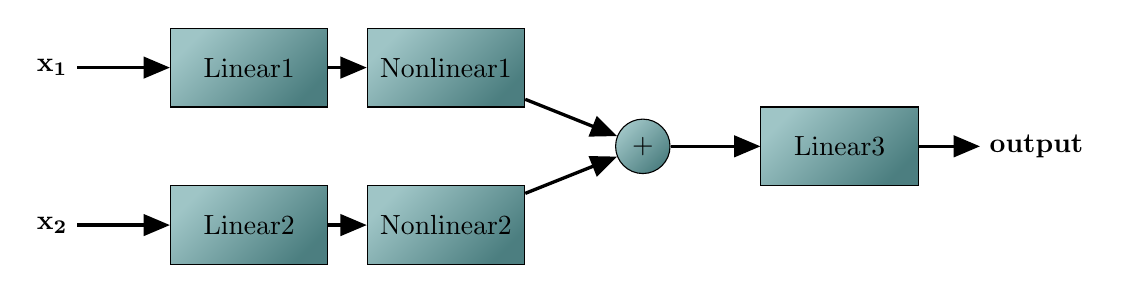
\begin{tikzpicture}
    %%Create a style for the arrows we are using
    \tikzset{normal arrow/.style={draw,-triangle 45,very thick}}
    %%Create the different coordinates to place the nodes
    \coordinate (1) at (0,0);
    \coordinate (2) at (2.5,0);
    \coordinate (3) at (2.5,-2);
    \coordinate (4) at (0,-2);
    \coordinate (5) at (5,-1);
    \coordinate (6) at (7.5,-1);
    \coordinate (x1) at (-2.5,0);
    \coordinate (x2) at (-2.5,-2);
    \coordinate (out) at (10,-1);
    %% Draw nodes
        \node[draw,rectangle,shading=axis,top color=CadetBlue!60, bottom color=CadetBlue!80!black,shading angle=45,minimum width = 2cm, minimum height = 1cm] (n1) at (1) {Linear1};
        \node[draw,rectangle,shading=axis,top color=CadetBlue!60, bottom color=CadetBlue!80!black,shading angle=45,minimum width = 2cm, minimum height = 1cm] (n2) at (2) {Nonlinear1};
        \node[draw,rectangle,shading=axis,top color=CadetBlue!60, bottom color=CadetBlue!80!black,shading angle=45,minimum width = 2cm, minimum height = 1cm] (n3) at (3) {Nonlinear2};
        \node[draw,rectangle,shading=axis,top color=CadetBlue!60, bottom color=CadetBlue!80!black,shading angle=45,minimum width = 2cm, minimum height = 1cm] (n4) at (4) {Linear2};
         \node[draw,circle,shading=axis,top color=CadetBlue!60, bottom color=CadetBlue!80!black,shading angle=45] (n5) at (5) {+}; 
         \node[draw,rectangle,shading=axis,top color=CadetBlue!60, bottom color=CadetBlue!80!black,shading angle=45,minimum width = 2cm, minimum height = 1cm] (n6) at (6) {Linear3};         
        \node (nx1) at (x1) {$\mathbf{x_1}$};
        \node (nx2) at (x2) {$\mathbf{x_2}$};
        \node (xout) at (out) {$\mathbf{output}$};
    %%Drawing the arrows
    \path[normal arrow] (nx1) -- (n1);
    \path[normal arrow] (nx2) -- (n4);
    \path[normal arrow] (n1) -- (n2);
    \path[normal arrow] (n4) -- (n3);
    \path[normal arrow] (n2) -- (n5);
    \path[normal arrow] (n3) -- (n5);
    \path[normal arrow] (n5) -- (n6);
    \path[normal arrow] (n6) -- (xout);
  \end{tikzpicture}
  \caption{Example of network that can be represented using our library.}
  \label{example_graph}
  \end{center}
\end{figure}  

\subsection{General Network}


% Modules
\subsection{Modules}
With the term \emph{module} we mean each possible element of the network from linear or nonlinear layers to the loss function. 
Moreover, other operators such as the sum of two different inputs are treated as modules, and hence we obtain an easier representation for more complex networks 3 .
The general structure of a module object is given in \verb|ModuleBase.py| and in each derived object we have to define the following methods:
\begin{itemize}
\item \verb|forward|: Implement the forward pass given the input of the module and store both the input and the output as attributes of the class. 
\item \verb|backward|: Compute the gradient of the loss with respect to the input given the gradient of the loss with respect to the output. If the module contains parameters, it also computes the gradient of the loss with respect of them.
\item \verb|update_param|: Given a learning rate as input, updates the parameters of the module using a gradient descent based approach.
\end{itemize}
\subsubsection{Linear Layer}



% Num 
\section{Numerical Experiments}\label{sec_numexp}
% simple model on linear data
Before running the model presented in the previous section, we run few simpler ``sanity check'' tests.
We first consider a simpler problem: a two-class classification problem where the discriminant line that separates  points classified with label 0 or 1 is  linear. 
In particular, we sample  points from a standard Normal distribution and assign them a soft label 0.8 or 0.2 if they lie on the left or on the right of a line with intercept in the origin and slope equal 4. 
To train this problem, we use a simple network where the operators and connectivity map are chosen as follows:
\begin{align*}
\text{operators} =  \{  & 1  \: :  \text{ Linear }, \\
&  2  \: : [\text{ Nonlinear }], \\
%   , 1  \: :  \text{ Linear3 } 
 \}.\\ 
\end{align*}
In this model the first value $ \text{ Linear }$ has dimensions number of classes $\times$ number of inputs [TODO controlla qui... sono dimensioni ? � giusto?] and the second value  $\text{ Nonlinear }$ is given by the Tanh function.
As shown in Figure \ref{fig_lin_results}, even a very simple network of this kind can provide satisfactory results on unseen data: 0.3\% error on the training dataset and 0.5\% error on the test set. 
 %Fig2
  \begin{figure}[h]
 \begin{center}
\begin{tabular}{l r}
  \includegraphics[width=0.5\textwidth]{fig/fig_linear_simplemodel_03err_train} & 
  \includegraphics[width=0.5\textwidth]{fig/fig_linear_simplemodel_05err_test} \\
  \end{tabular}
   \caption{Training (left) and test (right) sets for the first simple problem. The discriminant between the two classes is a line, points belonging to class 0 and 1 are marked in blue and red, respectively. Points misclassified are marked with a black x symbol.  \label{fig_lin_results}}
  \end{center}
  \end{figure}
  % End of fig2
  
For this problem and all the following once we sampled 1000 points in the train set and 200 points in test set. 
The learning rate is set equal to $0.05$ for all problems. 

As expected, this simple model does not generalise to more complex classification problems, where there discriminant lplane is non linear. 
This corresponds to the case we were asked to test: classify  randomly generated points  in $[0,1]^2$ with label 0 if they lie inside the circle of radius $\sqrt{2 \pi}^{-1}$ or 1 otherwise. 
For this setup a network with logistic sigmoids or Tanh is needed to learn the non-linearities.
Figure \ref{fig_circle} shows the results on an unseen test set.

% Conclusion
 \section{Conclusion}\label{sec_conclusion}
 
 
 % References
\bibliographystyle{abbrv}
\bibliography{mybib_dl} 
  
  
  
\end{document}